

% -----------------------------------------------------------------------------
\section{Privacy}
\label{s:Privacy}

\begin{figure}
\begin{center}
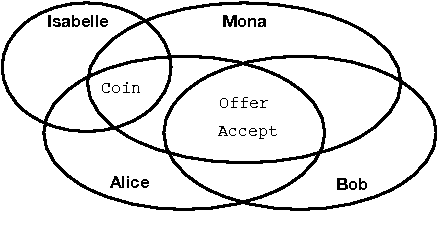
\includegraphics{figure/coin-transfer-visibility.pdf}
\end{center}
\vspace{-2ex}
\caption{Fact Visibility for Monitored Coin Transfer}
\label{f:CoinTransferVisibility}
\end{figure}

In practical multi-party workflows it is often not desirable, or even legal, for all data used in the workflow to be provided to all parties. In the coin transfer example from \S\ref{s:FactsWeights}, we could assume that Alice did not want to reveal the total number of coins she holds to Bob, nor the item she wishes to purchase (the Guitar) to Isabelle. Conversely, sometimes the details of a workflow \emph{must} be revealed to third parties that do not otherwise participate in that workflow. Details of transactions may need to be sent to financial regulators that monitor the operation of markets, or to credit agencies that offer loans based on the spending patterns of their clients. For the sake of example, we extend the coin transfer workflow described in the previous section with an extra party, Mona, who monitors all coin transactions. Figure~\ref{f:CoinTransferVisibility} describes fact visibility for the new workflow as a Venn diagram. The extended transfer rule is as per Figure~\ref{f:CoinTransfer}, but with Mona listed as an observer of the produced coin fact.


% -----------------------------------------------------------------------------
\subsection{Transaction and Validation}
\label{s:Transactions}
Assume that Alice, Bob, Mona and Isabelle all have their own computers in their own offices, each containing a \emph{fragment} of the ledger state as per Figure~\ref{f:CoinTransferVisibility}. Each party also has a copy of the extended transfer rule. Alice decides that it is time to perform the transfer, and builds the following transaction structure:

\begin{small}
\begin{code}
Transaction
 seq    = ... sequence number ...
 rule   = ... hash of the transfer rule ...
 input  = [ Offer [id = '1234, terms = "To purchase a Guitar",
                   giver = !Alice, receiver = !Bob]
            by  {!Alice}            obs {!Mona, !Bob}
            use {'transfer}         num  1

          , Accept [id = '1234, accepter = !Bob]
            by  {!Bob}              obs {!Mona, !Alice}
            use {'transfer}         num 1

          , Coin   [issuer = !Isabelle, holder = !Alice]
            by  {!Isabelle, !Alice} obs {!Mona}
            use {'transfer}         num 1 ]

 output = [ Coin   [issuer = !Isabelle, holder = !Bob]
            by  {!Isabelle, !Bob}   obs {!Mona}
            use {'transfer}         num 1 ]
\end{code}
\end{small}

\eject{}
The transaction includes a fresh sequence number, the hash of the transfer rule definition, the list of facts being consumed (input) by the transaction, and the list of new fact created (output). Alice would like the other parties to agree that this is a valid execution of the transfer rule, and update their own local fragments of the ledger state. However, as per Figure ~\ref{f:CoinTransferVisibility}, not all parties are entitled to see all facts listed in the transaction.

Recall from \S\ref{s:Observation} that a party $P$ can see a fact $F$ when it is listed in either its \emph{by-authority} set or its \emph{obs-authority} set. We express this as a predicate, where the functions \trm{auth-by} and \trm{auth-obs} retrieve the corresponding sets from the fact value.
$$
\trm{sees}~ P~ F = (P \in \trm{auth-by}~F) \lor (P \in \trm{auth-obs}~F)
$$
Applying this predicate to the facts in the transaction, Alice computes that 1) the @Offer@ and @Accept@ should be visible to Alice, Bob and Mona; 2) the input @Coin@ fact should be visible to Isabelle, Alice and Mona, and 3) the output @Coin@ fact should be visible to Isabelle, Bob and Mona. Importantly, the details of the transaction do not reveal how many coins Alice happens to have when she builds it. Both Isabelle and Mona will already know how many coins Alice has, as they have seen previous coin transfers, but there is no reason for this information to appear in the transaction structure itself.

Alice cannot send the complete transaction to all parties as they are not all entitled to see all the facts. Instead, Alice computes a \emph{restricted view} of the transaction for each of the other parties, blinding the facts that a particular party is not entitled to see from their view before sending it.


% -----------------------------------------------------------------------------
\subsection{Transaction Views}
We abbreviate the four weighted facts in the transaction structure as $d_1, d_2, d_3, d_4$. The letter $d$ is a mnemonic for \emph{factoid} --- being an ``unreliable'' fact, because the weight might be zero. We express the complete transaction as the following tuple, using $h(X)$ to mean the hash of value $X$, and $tx$ to denote the name of the transfer rule:
$$
 (seq,~ h(tx), [d_1, d_2, d_3], [d_4])
$$
This tuple contains the transaction sequence number, the hash of the rule definition, the list of input factoids, and the list of output factoids. The views for each party are computed by replacing some of the factoids by their \emph{blinded hashes}. A blinded hash is a cryptographic hash which has been combined with a random salt value, so that the plaintext data cannot feasibly be recovered by brute force guessing. We write $s_1 .. s_4$ as the salts for each factoid.

Before computing the view for each party, Alice first computes an overall transaction identifier by replacing all factoids in the transaction with their blinded hashes, then hashing the result:
$$
\begin{array}{rl}
 \hspace{-2ex} h((seq,~ h(tx), [h(d_1, s_1), h(d_2, s_2), h(d_3, s_3)], [h(d_4, s_4)]))
\end{array}
$$
This is a unique(ish) identifier for the transaction, provided the hash values are long enough that we will not see a collision in practice.

Now, as Isabelle is entitled to see the @Coin@ facts but not the @Offer@ or @Accept@ facts, she receives a view containing the data and salt values for the @Coin@ facts, but only the blinded hashes of the @Offer@ and @Accept@ facts:
$$
\trm{for Isabelle:}~~(seq,~ h(tx), [h(d_1, s_1), h(d_2, s_2), (d_3, s_3)], [(d_4, s_4)])
$$
Similarly, Bob is entitled to see the @Offer@, @Accept@ and produced @Coin@ fact, but not the consumed @Coin@ fact, so receives a corresponding view.
$$
\trm{for Bob:}~~(seq,~ h(tx), [(d_1, s_1), (d_2, s_2), h(d_3, s_3)], [(d_4, s_4)])
$$
Finally, Mona is entitled to see all the facts, so she gets the full unblinded transaction.
$$
\trm{for Mona:}~~(seq,~ h(tx), [(d_1, s_1), (d_2, s_2), (d_3, s_3)], [(d_4, s_4)])
$$
All four parties, including Alice, can now use their own view to compute the same transaction identifier. Isabelle was not given the data for the @Offer@ or @Accept@ facts, but as she knows their blinded hashes she can still compute the hash of the overall transaction. Isabelle \emph{can} infer that the giver and receiver fields of the @Offer@ must have contained values @!Alice@ and @!Bob@ respectively. Isabelle knows which rule the transaction has been generated from, and that rule says the giver and receiver of an @Offer@ must match the corresponding fields of the @Coin@ facts that she does see. However, Isabelle cannot see that the coin is being transferred @"To purchase a Guitar"@, because this information was only present in the @Offer@.


% -----------------------------------------------------------------------------
\subsection{Consensus}
Once each party has received their own transaction view, they can compare it against their own fragment of the ledger state and confirm with each other whether their views are valid. The fragment of ledger state visible to Isabelle includes the total weight of @Coin@ facts currently held by Alice. When Bob confirms with Isabelle that her view is valid, this tells Bob whether Alice actually has a coin to transfer to him. Similarly, when Isabelle confirms with Bob that his view is valid, this tells Isabelle that Bob really did agree to the transfer. In a practical workflow Isabelle might represent a commercial Bank, and in this case Bob would likely trust Isabelle to answer truthfully when asked if enough coins are available for a transfer, even though he does not want her to know that he is adding to his collection of guitars.

Consensus for the Rainfall model could be implemented in several different ways. For a small number of parties, such as to manage commercial workflows between banks, it would be sufficient for each party to confirm the transaction directly with all others. This would require $O(n^2)$ confirmations, but in the happy case the only information that needs to be exchanged is that the confirming party agrees with the transaction view identified by its hash code. For a greater number of parties, cryptographically signed confirmation messages could be propagated with a peer-to-peer protocol~\cite{El-Ansary2003:Broadcast}, or Byzantine Fault Tolerant (BFT) consensus protocol~\cite{Lamport1982:Byzantine, Ongaro2014:Consensus, Gilad2017:Algorand}. Both Corda~\cite{Hearn2016:Corda} and Hyperledger Fabric~\cite{Androulaki2018:Fabric} are existing networking frameworks that can be configured with custom transaction validation routines.

Alternatively, @Mona@ could represent a monitoring company that simply receives transaction views and archives them. In applications where the parties know each other and are expected to be honest, they may not need to synchronously confirm every transaction. If there are any disputes between Alice, Bob or Isabelle, then they could retrieve the complete views given to Mona, and validate that the transaction hashes of those views match their own.

\eject{}
% -----------------------------------------------------------------------------
\subsection{Nested Transactions}
\label{s:NestedTransactions}
For the transaction in \S\ref{s:Transactions}, Isabelle's view is constructed by blinding the @Offer@ and @Accept@ facts, as Isabelle is not entitled to see them. Blinding these facts means that Isabelle cannot use the input list to directly execute the rule and check its output. In a concrete implementation with a trusted monitor, such as Mona, this would not matter as the other parties would expect Mona to answer truthfully when asked if the transaction is valid. If we instead wish Isabelle to be able to validate the output directly, then we can split the transfer rule into two parts: one that combines Alice's offer with Bob's agreement, and another to perform the actual transfer.

\begin{small}
\begin{code}
  rule  agreeOffer
  await Offer  [id = ?i, giver = ?g, receiver = ?r] gain {g}
    and Accept [id = i,  accepter = r]              gain {r}
  to
    say Agreed [giver = g, receiver = r]
     by {g,r}  obs {!Mona,!Isabelle} use {'performTransfer}

  rule  performTransfer
  await Agreed [giver = ?g, receiver = ?r]        gain {g,r}
   and  Coin   [issuer = !Isabelle, holder = g]
        gain {!Isabelle,g}
  to
    say Coin   [issuer = !Isabelle, holder = r]
     by {!Isabelle,r} obs {!Mona} use ...
\end{code}
\end{small}

With these two rule definitions Alice can build a \emph{nested transaction}~\cite{Moss1981:Nested}, which for our purposes is a list containing the subtransaction for each of the rule firings. For the above rules, the first subtransaction will consume the @Offer@ and @Accept@ facts to produce an intermediate @Agreed@ fact that is authorized by both Alice and Bob. The second subtransaction will then immediately consume this @Agreed@ fact along with the input @Coin@ fact, to produce the output @Coin@ fact. Both the @Agreed@ fact, as well as the input @Coin@ fact are guaranteed to be visible to Isabelle, so she will be able to re-execute the second subtransaction and validate the output herself. Isabelle will not be able to see the terms of the offer, but she will be able to confirm with Bob that he agreed to it.

In related work, the DAML~\cite{DA2019:DAML} ledger model combines facts and rules into a \emph{contract instance}, similar to an object in an OO model --- where our facts would be the object's fields, and our rules its methods. Parties using the system authorize whole objects, instead of using separate systems for the authorization of facts (our by-authority set) and rules (our use-set). DAML is based on UTxO~\cite{Zahnentferner2018:UTxO}, so calling a method on an object typically causes it to allocate some new objects and consume the called object.

A design decision of DAML is to ensure that each party who authorizes an object is able to re-execute the subtransaction that consumes that object. Supporting this requires the system to sometimes \emph{divulge} additional objects to an authorizing party that were not visible until the object they authorized was consumed. However, the object oriented code structure of DAML causes the transactions produced by method invocation to have a nested form similar to the above. In DAML, the details of the equivalent @performTransfer@ subtransaction can be sent to @Isabelle@, leaving the details of @agreeOffer@ private between Alice and Bob.


% -----------------------------------------------------------------------------
\subsection{Incidental Observers}
For the transaction from \S\ref{s:Transactions}, although Alice was the one that formed this transaction, she herself is not listed as an observer of the output @Coin@ fact. When Alice computes the restricted views for Bob, Isabelle and Mona she knows that those parties will add this output fact to their own stores, but she should not add it to her own. As Alice is not an observer of the output fact, any other party that builds a transaction that consumes this fact will not inform her that this has happened. In this case we say that Alice is an \emph{incidental observer} of the output @Coin@ fact.


% -----------------------------------------------------------------------------
\begin{figure}
\begin{center}
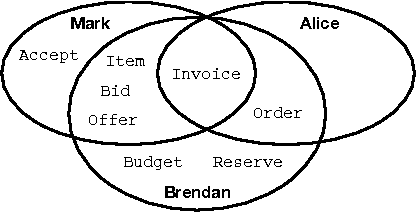
\includegraphics{figure/auction-visibility.pdf}
\end{center}
\vspace{-2ex}
\caption{Fact Visibility for Market Example}
\label{f:AuctionVisibility}
\end{figure}


\subsection{Fact Selection and Checking}
\label{s:Query}
\label{s:Selection}
In the coin transfer rules discussed so far, each pattern matching clause only gathered a single fact at a time. Consider instead a market workflow where rules must perform more complex queries, such as selecting the cheapest item that matches some criteria. Figure~\ref{f:AuctionVisibility} shows the fact visibility for an example workflow. Mark runs the market, Brendan is a broker, and Alice is a client who wishes to buy some items. Alice must interact with Mark through Brendan, instead of communicating directly, like so:

\begin{enumerate}
\item Mark maintains @Item@ facts that describe items available for sale, along with their asking price. Brendan can pay the asking price to buy an item immediately, or bid below the asking price, which Mark may or may not accept.

\item Alice creates @Order@ facts describing the sort of items she wishes to buy, her price limit per item, and her total budget for items of this sort. Brendan can see Alice's @Order@ facts, but Mark naturally cannot, as Alice does not want Mark to know the maximum price she is willing to pay.

\item Brendan attempts to fulfill Alice's orders by bidding on multiple items concurrently. Brendan maintains a local @Budget@ fact recording how much of Alice's total budget has not yet been committed to bids. This ensures he does not accidentally bid on items that Alice is not prepared to pay for.

\item When Brendan wishes to enter a new bid he creates a local @Reserve@ fact, which indicates that some of Alice's budget needs to be reserved for this bid. This causes one of Brendan's business rules to fire, which first checks that enough @Budget@ is available, and if so, subtracts from the current @Budget@, then sends an active @Bid@ to Mark.

\item On Mark's side, one of Mark's business rules finds the cheapest available @Item@ that matches the description in Brendan's @Bid@, and if the bid price is lower than the ask price, converts the bid to an outstanding @Offer@.

\item Later, if Mark decides to accept Brendan's lower offer, then Mark creates a local @Accept@ fact. One of Mark's business rules matches the @Accept@ with the corresponding @Offer@ and @Item@, consumes all three, and creates an @Invoice@ which is visible to all three parties.
\end{enumerate}

An interesting aspect of this workflow is that different parties in the system will naturally want to maintain their own local business rules, and corresponding fact declarations. The way Brendan accounts for bids he has placed on Alice's behalf is of no concern to Mark, but expressing all rules in the same framework means they can communicate directly. Here is the rule Brendan uses to check the @Budget@ and produce a @Bid@.

\begin{small}
\begin{code}
  fact Item    [lot:  Nat,  desc:   Text, ask: Nat]
  fact Bid     [lot:  Nat,  offer:  Nat]
  fact Order   [desc: Text, limit:  Nat,  budget: Nat]
  fact Budget  [desc: Text, total:  Nat,  remain: Nat]
  fact Reserve [lot:  Nat,  bid:    Nat]

  rule  reserve
  await Order   [desc  = ?d, limit  = ?l]
        consume none                      gain  {!Alice}
    and Item    [lot   = ?o, desc   = d,  ask = ?a]
        select first a   consume none     check {!Mark}
    and Budget  [total = ?t, remain = ?m] gain  {!Brendan}
    and Reserve [lot   = o,  bid    = ?b]
        where b <= l && b <= a && b <= m  gain  {!Brendan}
   to union
    (say Budget  [desc  = d,  total = t,  remain = m - a]
        by {!Brendan}  use ...)
    (say Bid     [lot   = o,  price  = a]
        by {!Brendan, !Alice}  obs {!Mark}  use ... })
\end{code}
\end{small}

The @Order@ pattern has a @consume none@ clause to indicate that we only want to read the fact data, rather then consume any weight of it, as the complete order might not be fulfilled yet. The @Order@ pattern does not mention the @budget@ field as this particular rule does not use it. The @Item@ pattern has a @select first a@ clause to indicate that all items that match the description in the order should be sorted by the asking price @a@, and the first one selected. Brendan should only bid on the cheapest matching item available. The @Reserve@ pattern has a @where@ clause to check the bid being placed is no more than Alice's price limit, no more than the market asking price, and no more than the remaining budget for Alice.

When the rule matches on its facts it will @gain@ the authority of the client and broker. The output @Budget@ only needs to be authorized by Brendan as this is his internal accounting. The output @Bid@ is authorized jointly by Brendan and Alice, as Brendan is entering the bid on behalf of Alice. Finally, in the pattern for @Item@, the rule @check@s that this fact has been authorized by Mark rather than trying to @gain@ his authority. The @check@ clause allows patterns to match on observable facts without the rule name being mentioned in the use-set of that fact. Mark should not need to concern himself with Brendan's accounting, so the @Item@ facts that Mark creates do not need to mention Brendan's rules. Brendan's @reserve@ rule can still execute because it is not consuming any facts authorized by Mark, or producing any that are authorized in his name.


% -----------------------------------------------------------------------------
\subsection{Upgrade}
\label{s:Upgrade}
As a final example, in practical workflows it is necessary to upgrade data formats and business rules as requirements change. In Rainfall, upgrading workflows is easy as the use-sets attached to each fact can be manipulated directly:

\begin{small}
\begin{code}
  rule   upgrade
  await  Coin [issuer = ?s, holder = ?h]      gain {s,h}
     and LetsUpgrade [party = s, rules = ?rs] gain {s}
     and LetsUpgrade [party = h, rules =  rs] gain {h}
  to say Coin [issuer = s, holder = h]
      by {s,h} use rs
\end{code}
\end{small}

This rule allows the issuer and holder of a @Coin@ to jointly agree to change the fact's use-set, and the new use-set can mention new versions of existing rules. There is no need for a privileged operator party to orchestrate the upgrade. The meaning of facts is controlled by the parties that authorize them, and not the people that operate the ledger system.


